
\documentclass[10pt,a4paper]{article}
\usepackage[T1]{fontenc}
\usepackage{tikz}
\usepackage[margin=1cm]{geometry}
\begin{document}
\section*{AVL Tree Algorithm Overview}

An AVL tree is a self-balancing binary search tree where the height difference between the left and right subtrees of any node is at most one. This balance ensures that the tree remains approximately balanced, leading to $O(\log n)$ time complexity for search, insertion, and deletion operations.

\subsection*{Key Concepts}
\begin{itemize}
    \item \textbf{Height}: The height of a node in an AVL tree is the length of the longest path from the node to a leaf. This height is used to determine the balance of the node.
    \item \textbf{Balance Factor}: For any node in the AVL tree, the balance factor is calculated as the height of the left subtree minus the height of the right subtree. It helps in determining if the node is balanced, left-heavy, or right-heavy.
    \item \textbf{Rotations}: To maintain balance in the AVL tree after insertions and deletions, rotations are performed. There are four types of rotations:
    \begin{itemize}
        \item \textbf{Right Rotation (Single Rotation)}: Applied when a left-heavy subtree needs balancing.
        \item \textbf{Left Rotation (Single Rotation)}: Applied when a right-heavy subtree needs balancing.
        \item \textbf{Left-Right Rotation (Double Rotation)}: Applied when a left subtree has a right-heavy child.
        \item \textbf{Right-Left Rotation (Double Rotation)}: Applied when a right subtree has a left-heavy child.
    \end{itemize}
\end{itemize}

\subsection*{Initial AVL Tree}
\begin{center}
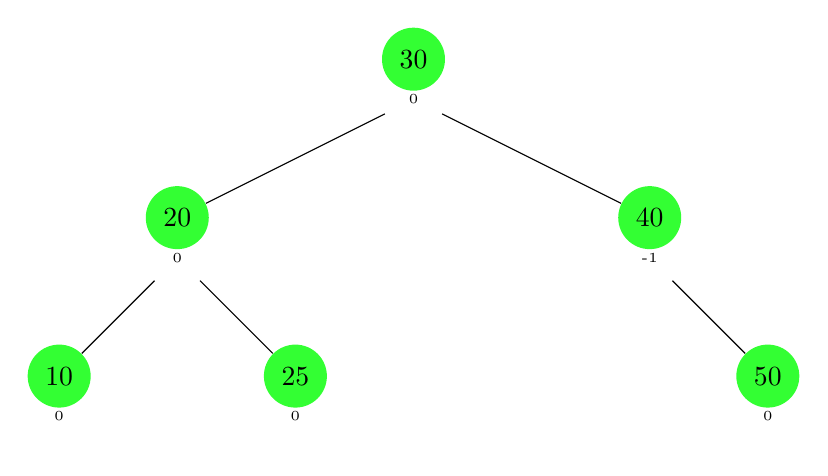
\begin{tikzpicture}[level distance=15mm, sibling distance=20mm]
    \tikzstyle{every node}=[circle,inner sep=1pt, minimum size=8mm]
    \tikzstyle{level 1}=[sibling distance=60mm]
    \tikzstyle{level 2}=[sibling distance=30mm]
    \tikzstyle{level 3}=[sibling distance=15mm]
    \tikzstyle{level 4}=[sibling distance=10mm]
    \node [fill=green!80] {30} node [below=3pt] {\tiny 0} child {node [fill=green!80] {20} node [below=3pt] {\tiny 0} child {node [fill=green!80] {10} node [below=3pt] {\tiny 0} } child {node [fill=green!80] {25} node [below=3pt] {\tiny 0} }} child {node [fill=green!80] {40} node [below=3pt] {\tiny -1} child[fill=none] {edge from parent[draw=none]} child {node [fill=green!80] {50} node [below=3pt] {\tiny 0} }};
\end{tikzpicture}
\end{center}

\subsection*{Final AVL Tree}
\begin{center}
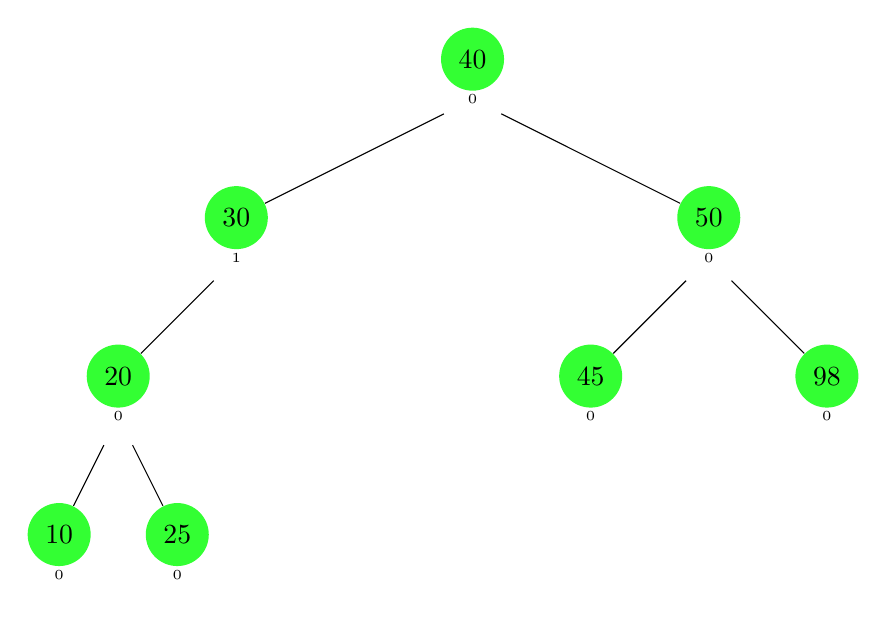
\begin{tikzpicture}[level distance=15mm, sibling distance=20mm]
    \tikzstyle{every node}=[circle,inner sep=1pt, minimum size=8mm]
    \tikzstyle{level 1}=[sibling distance=60mm]
    \tikzstyle{level 2}=[sibling distance=30mm]
    \tikzstyle{level 3}=[sibling distance=15mm]
    \tikzstyle{level 4}=[sibling distance=10mm]
    \node [fill=green!80] {40} node [below=3pt] {\tiny 0} child {node [fill=green!80] {30} node [below=3pt] {\tiny 1} child {node [fill=green!80] {20} node [below=3pt] {\tiny 0} child {node [fill=green!80] {10} node [below=3pt] {\tiny 0} } child {node [fill=green!80] {25} node [below=3pt] {\tiny 0} }} child[fill=none] {edge from parent[draw=none]}} child {node [fill=green!80] {50} node [below=3pt] {\tiny 0} child {node [fill=green!80] {45} node [below=3pt] {\tiny 0} } child {node [fill=green!80] {98} node [below=3pt] {\tiny 0} }};
\end{tikzpicture}
\end{center}

\end{document}
